\documentclass[a4 paper]{article}
\usepackage[inner=2.0cm,outer=2.0cm,top=2.5cm,bottom=2.5cm]{geometry}
\usepackage{setspace}
\usepackage[T2A]{fontenc}
\usepackage[utf8]{inputenc} 
\usepackage[russian, english]{babel}
\usepackage[rgb]{xcolor}
\usepackage{verbatim}
\usepackage{subcaption}
%стиль вставки кода
\usepackage{pythonhighlight}

\usepackage{amsgen,amstext,amsbsy,amsopn,tikz,amssymb,tkz-linknodes}
\usepackage{amsmath,amsthm,amssymb,amsfonts}
\usepackage{fancyhdr}
\usepackage[colorlinks=true, urlcolor=blue,  linkcolor=blue, citecolor=blue]{hyperref}
\usepackage[colorinlistoftodos]{todonotes}
\usepackage{rotating}
%настройка вставки рисунков
\usepackage{graphicx}
\graphicspath{{pictures/}}
\DeclareGraphicsExtensions{.pdf,.png,.jpg}

\hypersetup{%
pdfauthor={Ashudeep Singh},%
pdftitle={Homework},%
pdfkeywords={Tikz,latex,bootstrap,uncertaintes},%
pdfcreator={PDFLaTeX},%
pdfproducer={PDFLaTeX},%
}
\usepackage{booktabs}
\newcommand{\ra}[1]{\renewcommand{\arraystretch}{#1}}

\theoremstyle{definition}
\newtheorem{defin}{Определение}

\theoremstyle{plain}
\newtheorem{thm}{Теорема}
\newtheorem{prop}{Утверждение}
\newtheorem*{ext}{ }

\theoremstyle{remark}
\newtheorem*{prf}{Доказательство}
\newtheorem*{remark}{Примечание}

\newcommand{\specialcell}[2][c]{%
  \begin{tabular}[#1]{@{}c@{}}#2\end{tabular}}

\newcommand{\homework}[6]{
   \pagestyle{myheadings}
   \thispagestyle{plain}
   \newpage
   \setcounter{page}{1}
   \noindent
   \begin{center}
   \framebox{
      \vbox{\vspace{2mm}
    \hbox to 6.28in { {\bf OzonMasters - Математическая статистика \hfill {\small (#2)}} }
       \vspace{3mm}
       \hbox to 6.28in { {\Large \hfill #1  \hfill} }
       \vspace{3mm}
       \hbox to 6.28in { {\it Преподаватель: {\rm #3} \hfill Автор конспекта: {\rm #5}}}
       %\hbox to 6.28in { {\it TA: #4  \hfill #6}}
      \vspace{1mm}}
   }
   \end{center}
   \markboth{Математическая статистика -- #1}{Математическая статистика -- #1}
   \vspace*{1mm}
}

\newcommand{\problem}[1]{~\\\fbox{\textbf{Условие #1}}\newline\newline}
\newcommand{\subproblem}[1]{~\newline\textbf{(#1)}}
\newcommand{\D}{\mathcal{D}}
\newcommand{\Hy}{\mathcal{H}}
\newcommand{\VS}{\textrm{VS}}
\newcommand{\solution}[1]{~\\\fbox{\textbf{Решение #1}}\newline}


\newcommand{\bbF}{\mathbb{F}}
\newcommand{\bbX}{\mathbb{X}}
\newcommand{\bI}{\mathbf{I}}
\newcommand{\bX}{\mathbf{X}}
\newcommand{\bY}{\mathbf{Y}}
\newcommand{\bepsilon}{\boldsymbol{\epsilon}}
\newcommand{\balpha}{\boldsymbol{\alpha}}
\newcommand{\bbeta}{\boldsymbol{\beta}}
\newcommand{\0}{\mathbf{0}}


\begin{document}
\homework{Лекция 1}{Due: 18/09/20}{Владимир Панов}{}{Жибоедова Анастасия}

\section{Рекомендуемая литература}
\begin{enumerate}
    \item М.Б. Лагутин "Наглядная математическая статистика"
    \item Robert Hogg, Elliot Tanis, Dale Zimmerman "Probability and Statistical Inference"
    \item Yuri Suhov, Mark Kelbert "Basic Probability and Statistics" 
    \item Vladimir Spokoiny, Thorsten Dickhaus "Basics of Modern Mathematical Statistics" 
\end{enumerate}

\section{Статистический эксперимент}

\subsection{Описание статистического эксперимента}
Введем некоторые опредления для дальнейшего описания эксперимента с математической строгостью.
\begin{defin}
$\Omega$ - sample space, множество элементарных исходов.
\end{defin}
\begin{defin}
$\mathcal{F}$ - $\sigma$-алгебры - множество подмножество пространства $\Omega$, обладающее следующими свойствами:
\begin{enumerate}
    \item $\emptyset, \Omega \in \mathcal{F}$
    \item $A \in \mathcal{F} \Rightarrow \Omega \backslash A \in \mathcal{F}$
    \item $A_1, A_2, \cdots \in \mathcal{F} \Rightarrow \cup A_i, \cap A_i \in \mathcal{F}$
\end{enumerate}
\end{defin}
\begin{defin}
Борелевская $\sigma$-алгебры - это минимальное множество 
\end{defin}
\begin{defin}
Вероятностная мера $\mathbb{P}: \mathcal{F} -> [0,1]$: 
\begin{enumerate}
    \item $\mathbb{P}\{\Omega\} = 1,$
    \item $A_i, A_2 \cdots \in \mathcal{F}, A_i \cap A_j = \emptyset \Rightarrow \mathbb{P}\{\cup A_i\} = \sum \mathbb{P}\{A_i\}$
\end{enumerate}
\end{defin}

Предположим, что вероятностная мера $\mathbb{P} \in \mathcal{P}$, если:
\begin{itemize}
    \item $\mathcal{P} = \mathcal{P}_{\theta} = \{\mathbb{P}_{\theta} \}$ - модель параметрическая;
    \item $\mathcal{P}$ - пространство бесконечной размерности,$\mathcal{P} = \{\text{абсолютно непрерывная}\}$ - непараметрическая модель.
\end{itemize}

\begin{defin}
Статистические эксперимент - это модель, задаваемая следующей тройкой параметров: $(\Omega, \mathcal{F}, \mathcal{P})$. $\Omega, \mathcal{F}$ - описывают как проводится эксперимент, а $\mathcal{P}$ - оценивается по итогам эксперимента. 
\end{defin}


\subsection{Примеры экспериментов}
Реконструируем модели стандартных статистических экспериментов: подбрасывание монеты и выбор случайной точки на отрезке.
\begin{table}[h]
    \centering
    \begin{tabular}{|c|c|p{0.43\linewidth}|p{0.31\linewidth}|}
        \hline
        Эксперимент &  $\Omega$ & $\mathcal{F}$ & $\mathbb{P}$\\
        \hline
        Бросание монеты &  $\{0,1\}$ & $\{ \emptyset, \{0\}, \{1\}, \{0,1\}\}$ & $\mathbb{P}\{1\}=p; \mathbb{P}\{0\} = 1-p$\\
        \hline
        Выбор точки на [0,1] & $[0,1]$ & 
        \specialcell{$
        \{ \{[a,b], 0 \leq a < b \leq 1\}, (a,b)  = \Omega \backslash([0,a] \cup [b,1]), \\\ 
        [a,b) = \cap (a - \frac{1}{n}, b), (a,b] = \cap (a, b + \frac1n) \\\ 
        \{a\} = [0,a] \cap [a,1] \}$ - Борелевская $\sigma$ -  алгебра}& \specialcell{$\mathbb{P} \{[a,b]\} = b-a$ - нет косоглазия, \\ иначе $\mathbb{P}$ - вер-ое распред. на [0,1]} \\
        \hline
    \end{tabular}
    \label{tab:my_label}
\end{table}

\section{Выборка (sample)}
\begin{defin}
(\textit{Простые учебники}) $x_1, \cdots x_n \in \mathbb{R}$ - выборка, это значения из набора случайных величин $X_1, \cdots X_n$ - i.i.d. (independent and identically distributed) с фиксированной $\omega \in \Omega$ (реализация случайных величин).
\end{defin}
\begin{remark}
На пространстве $(\Omega. \mathcal{F}, \mathbb{P})$ - нет независимых случайных величин, они либо тривиальны, либо зависимы. Чтобы провести статистический эксперимент, необходимо рассмотреть пространство $(\Omega \times \cdots \times \Omega), \mathcal{F} \times \cdots \times \mathcal{F}, \mathbb{P}: \mathbb{P}\{B \times \cdots\times B_n\} = \mathbb{P}_\theta(B_1) \cdot \cdots \cdot \mathbb{P}_\theta(B_n))$.
\end{remark}

\section{Описательная статистика (descriptive statistics)}
\begin{defin}
$x_{(1)} \leq \cdots \leq x_{(n)}$, где $x_{(1)} = min(x_1, \cdots x_n)$ - варианционный ряд, порядковые статистики
\end{defin}

\begin{defin}
Эсперическая $p$-квантиль - это такое число $x$, что:
\begin{itemize}
    \item $\approx np$ чисел $<x$
    \item $\approx np$ чисел $>x$
\end{itemize}
\end{defin}
\begin{remark}
Понятие описательных статистик вышло за рамки описания параметров. 
\end{remark}
\begin{defin}
Медиана - (самый известный квантиль) $\frac12$ - квантиль.
\begin{equation*}
Med = 
 \begin{cases}
   x_{(k)}, \text{если } n = 2k + 1 \\
   \dfrac{x_{(k)} + x_{(k + 1)}}{2}, \text{если } n =2k
 \end{cases}
\end{equation*}
\end{defin}

\subsection{Оценивание квантилей}

\subsubsection*{offtop}
Абсолютно непрерывные распредления, это такие распределения, что функция распредления имеет производную $F'(x) = p(x)$, где $p(x)$ - плотность распредления (probability density function).

Собирается статистика количества клиентов в магазине без понимания вида распределения. В случае, если распределение никаким образом не ограничивается параметрами, оно считается непараметрическим. 

Из определения квантиля можно увидеть то, что нам необходимо решить уравнение $F(x) = p$ (cumulative distribution function) - , где $\mathbb{P}\{X \leq x\}$. Решение уравнения возможно двумя способами: из книжек и из пакетов.

\subsubsection{Способ 1}
Теоретический способ решения уравнения. $\hat{F}_n (x)$ - empirical distribution function - оценка функции $F(x)$.
$$
\hat{F}_n (x) = \frac1n\sum_{i=1}^n \mathbb{I}\{X_i \leq x\}
$$
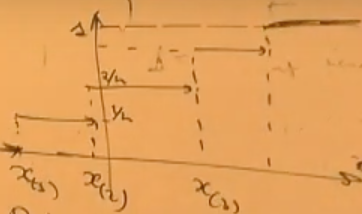
\includegraphics[scale=0.5]{F(x).png}
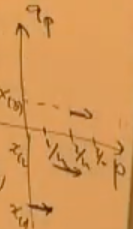
\includegraphics[scale=0.5]{q(p).png}

Решить уравнение из предположения $\hat{F}_n (x) = F(x)$, тогда $\hat{F}_n (x) = p$:
\begin{equation*}
x = q_p = 
 \begin{cases}
   x_{(pn)}, pn \in \mathbb{N} \\
   x_{(\lfloor pn \rfloor + 1)}, pn \notin \mathbb{N}
 \end{cases}
\end{equation*}
Иногда встречается упрощенная модификация решения (выборочная $\alpha$ - квантиль) $q_p = x_{(\lfloor pn \rfloor + 1)}$

Недостатком данного способа решения является то, что на выходе получается разрывная функция $q_p$.

\subsubsection{Способ 2}
Определим функцию следующим образом:
\begin{itemize}
    \item определим значения функций в наборе точек как - $(\frackn, x_{(k)}), k = 1, \cdots n$;
    \item доопределим функцию на отрезках линейными функциями.
\end{itemize}
В описанном подходе точки выбраны из значений функции эмперического распредления, но в пакетах используются иные значения. 

Построим последовательность $F(x_{(1)}),F(x_{(2)}) \cdots F(x_{(n)})$ - n чисел, являющихся реализациями случайных величин $F(X_{(1)}),F(X_{(2)}) \cdots F(X_{(n)})$. Поскольку функция $F(X_{(i)})$ - монотонно возрастающая, то можно трактовать это так, что послежовательность i.i.d случайных величин $F(X_{(1)}),F(X_{(2)}) \cdots F(X_{(n)})$ соответствует расположению в порядке возрастания случайных величин  $F(X_1),F(X_2) \cdots F(X_n)$. $\mathbb{P}\{F(X) \leq x\} = \mathbb{P}\{X \leq F^{-1}(x)\} = F(F^{-1}(x)) = x$, тогда с.в. $F(X_1),F(X_2) \cdots F(X_n)$ - имеют равномерные распредления.

Построим следующую цепочку выводов (без доказтельств):
\begin{itemize}
    \item $U_1 \cdots U_n - Unif([0,1])$ равномерно распределенные с.в.,
    \item тогда $U_{(i)} \sim Beta(i, n-i + 1)$ - $i$-ый член вариационного ряда
    \item тогда $p_i(x) = \dfrac{n!}{(i-1)!(n-i)!}x^{i-1}(1-x)^{n-i}$ плотность случайной величины $F(X_{(i))}$
    \item можно доказать, что $\mathbb{E}U_i = \mathbb{E}F(X_{(i)} = \dfrac{i}{n+1}$
    \item из вышесказанного следует, что в качестве опорных точек построения квантилей можно взять $(\frac{k}{n+1}, x_{(k)}), k = 1, \cdots n$ - реализация пакета spss (и др.).
\end{itemize}

Почему характерным значением называется среднее??? Оказывается, что это не совсем так.

\begin{defin}
Мода абсолютно непрерывного распределения - точка максимума плотности (наиболее модное значение).
\end{defin}

Во многих пакетах вместо среднего берется мода - $mode(U_i) = \frac{i-1}{n-1}$, соответственно в качестве опорных точек $(\frac{k - 1}{n-1}, x_{(k)}), k = 1, \cdots n$.
\end{document}



